\chapter{Special Continuous Random Variables}
\begin{definition}{}{}
  A continuous random variable \(X\) has a \emph{normal distribution} with mean \(\mu\) and standard deviation \(\sigma\), denoted by \(X \sim \operatorname{N}(\mu,\sigma^2)\), iff its pdf \(f\) is such that 
  \[f(x)=\frac{1}{\sigma\sqrt{2\pi}}\exp\left(-\frac{(x-\mu)^2}{2\sigma^2}\right).\]
\end{definition}
\begin{stbox}{General Information}
  \begin{itemize}
    \item A normal distribution is symmetrical about the line \(x=\mu\). That is 
    \[\Prob(X\leq\mu-\delta)=\Prob(X\geq\mu+\delta)\]
    for each \(\delta>0\). Note that the mean, median, and mode coincide with \(\mu\).
    \item Properties of the normal distribution. Let \(X\) and \(Y\) be independent, such that \(X \sim \operatorname{N}(\mu,\sigma^2)\) and \(Y \sim \operatorname{N}(m,s^2)\). Then, for any \(n \in \mathbb{N}\) and \(x\), \(y \in \mathbb{R}\),  
    \begin{itemize}
      \item \(nX \sim \operatorname{N}(n\mu,n^2\sigma^2)\),
      \item \(X_1+X_2+\cdots+X_n \sim \operatorname{N}(n\mu,n\sigma^2)\),
      \item \(aX\pm bY \sim \operatorname{N}(a\mu\pm bm,a^2\sigma^2+b^2s^2)\).
    \end{itemize}
    \item At times, the question may be phrased in a misleading manner. Try using some inference to figure out the intended interpretation.
  \end{itemize}
\end{stbox}
\begin{example}{}{}
  ``The mass of the padding is \(30\%\) of the mass of a randomly selected light bulb of mass \(L\). Find the probability that a light bulb with padding has mass \(c\).'' 
    
  Then for any light bulb of mass \(L_1\), the mass of the padding is \(0.3L_2\) (and \emph{not} \(0.3L_1\)). i.e. we are to find \(\Prob(L_1+0.3L_2)\).
\end{example}
\begin{stbox}{}
  \begin{itemize}
    \setcounter{enumi}{3}
    \item A variable \(Z\sim \operatorname{N}(0,1)\) is said to follow the \emph{standard} normal distribution.

    \emph{Note}: \(Z\) is reserved for this purpose.
    \item Let \(X \in \operatorname{N}(\mu,\sigma^2)\). Then, \(\frac{X-\mu}{\sigma}\) follows the standard normal distribution. 
    \item What \texttt{Tail} do we select for \texttt{invNorm}?
    \begin{center}
      \begin{tabular}{|Sc|Sc|}
        \hline
        \(\Prob(X<x)=p\) & \texttt{LEFT}\\
        \hline
        \(\Prob(-x<X<x)=p\) & \texttt{CENTER}\\
        \hline
        \(\Prob(X>x)=p\) & \texttt{RIGHT}\\
        \hline
      \end{tabular}
    \end{center}
    \item When using \texttt{invNorm} on an inequality, what should the sign be? For simplicity, we write \(\mathscr{L}(p)=\texttt{invNorm}(p,0,1,\texttt{RIGHT})\), and \(\mathscr{R}(p)=\texttt{invNorm}(p,0,1,\texttt{LEFT})\). Then,
    \begin{center}
      \begin{tabular}{|Sc|Sc|Sc|}
        \hline
        \(\Prob(Z>z)\geq p\) & \(z\leq \mathscr{L}(p)\)\\
        \hline
        \(\Prob(Z>z)\leq p\) & \(z\geq \mathscr{L}(p)\)\\
        \hline
        \(\Prob(Z<z)\geq p\) & \(z\geq \mathscr{R}(p)\)\\
        \hline
        \(\Prob(Z<z)\leq p\) & \(z\leq \mathscr{R}(p)\)\\
        \hline
      \end{tabular}
    \end{center}
  \end{itemize}
\end{stbox}
\begin{example}{}{}
  Suppose we want to find the least integer value of \(m\) for which \(\Prob(Z>1-m)\geq 1/2\).

  Then, using \texttt{invNorm (RIGHT)}, we infer that \(z\leq 0\), \emph{not} \(z\geq 0\). An illustration: 
  \begin{center}
    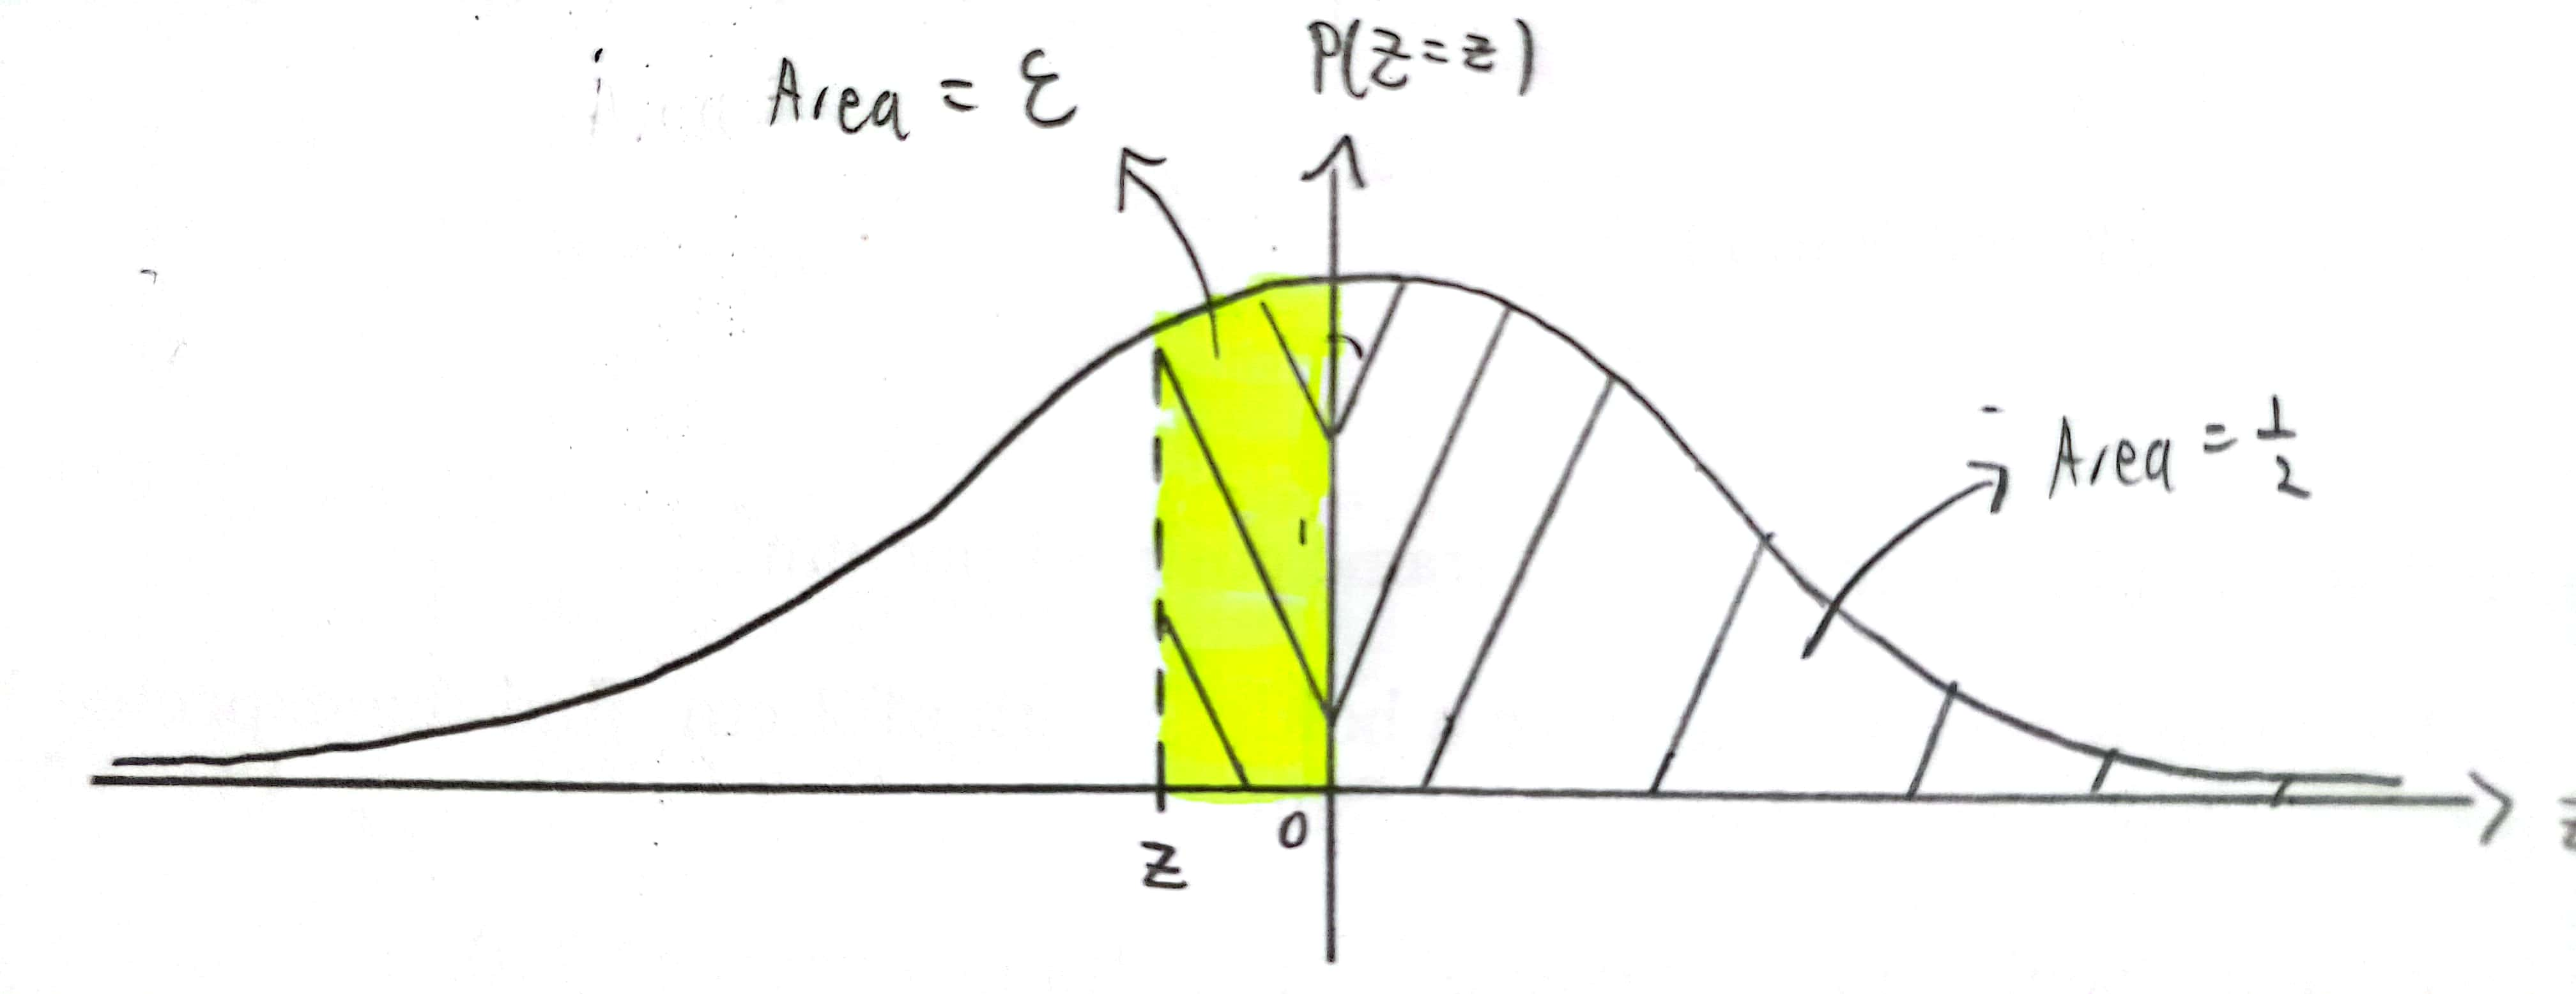
\includegraphics[width=\textwidth]{../images/Special-Continuous-Random-Variables-Example-Illustration.jpg}
  \end{center}
\end{example}
\begin{definition}{}{}
  A continuous random variable \(X\) has a \emph{uniform distribution} over the interval \((a,b)\), which is denoted by \(X \sim \operatorname{U}(a,b)\), iff its pdf \(f\) is such that
    \[f(x)=\begin{cases}
      \frac{1}{b-a} &\text{if \(a<x<b\),}\\
      0 &\text{otherwise.}
    \end{cases}\] 
\end{definition}
\begin{note}
  Let \(l\) and \(u\) be the lower and upper quartiles, of a normal distribution \(X\sim\Normal(\mu,\sigma^2)\). i.e. \(\Prob(X<l)=1/4\) and \(\Prob(X<u)=3/4\). Then, 
  \[P{\left( \mu-\highlight[yellow]{\frac{u-l}{2}}<X<\mu+\highlight[yellow]{\frac{u-l}{2}} \right)}=\Prob(l<X<u)=1/2.\]
\end{note}
\begin{definition}{}{}
  A continuous random variable \(Y\) has an (negative) exponential distribution, which we denote with \(Y\sim \operatorname{Exp}(\lambda)\), iff its pdf \(g\) is such that
    \[g(Y)=
    \begin{cases}
      \lambda e^{-\lambda x} &\text{if \(x\geq 0\)},\\
      0 &\text{otherwise.}
    \end{cases}\]
  (An exponential distribution models time between occurrences.)
\end{definition}
\begin{note}
  Let \(Y \sim \operatorname{Exp}(\lambda)\), then
  \[\Prob(Y>z+y \,\vert\, Y>y)=\Prob(Y>z) \qquad\text{and}\qquad\Prob(Y<z+y \,\vert\, Y>y)=\Prob(Y<z).\]
  % In general, it also holds that 
  % \[\Prob(V>z+y \,\vert\, V>y)=1-\Prob(V<z+y \,\vert\, V>y)\]
  % for any random variable \(V\).
\end{note}
\begin{stbox}{}
  \begin{itemize}
    \item Expectation and variance:
    \begin{center}
      \begin{tabular}{|Sc|Sc|Sc|}
        \hline
        Distribution & Expectation & Variance\\
        \hline
        \(X\sim \operatorname{U}(a,b)\) & \(\dfrac{a+b}{2}\) & \(\dfrac{(b-a)^2}{12}\)\\
        \hline
        \(Y\sim \operatorname{Exp}(\lambda)\) & \(\dfrac{1}{\lambda}\) & \(\dfrac{1}{\lambda^2}\)\\
        \hline
      \end{tabular} 
    \end{center}
    \emph{Note}: We need to remember the expectation and variance for the uniform distribution, as it is not provided in the MF26 formula sheet (unlike all other distributions).
    \item \emph{Warning}: The G.C. tends to incorrectly process an integral if its upper and lower bounds contain \(\pm \text{E}99\).
    \item Let \(T\) be the time taken between two consecutive arrivals and \(\#\sim\operatorname{Po}(\lambda t)\) the number of arrivals in time \(t\). Then, 
    \[\Prob(T>t)=\Prob(\#=0)=e^{-4t}.\]
    As such, the probability that there is at least one arrival in an interval of time \(t\) is 
    \[\Prob(T\leq t)=1-e^{-4t}.\]  
  \end{itemize}
\end{stbox}